\documentclass[AMA,STIX1COL,doublespace]{WileyNJD-v2}

\usepackage{longtable}


\usepackage{placeins}
\newcommand{\ie}{\textit{i.e., }}
\newcommand{\eg}{\textit{e.g., }}
\newcommand{\icv}{$\texttt{I}\!\!\rightarrow\!\texttt{CV}$}
\newcommand{\cvi}{$\texttt{CV}\!\circlearrowright\!\texttt{I}$}

\articletype{Research article}

\received{2020-xx-xx}

\revised{2020-xx-xx}

\accepted{2020-xx-xx}

\raggedbottom

\providecommand{\tightlist}{%
  \setlength{\itemsep}{0pt}\setlength{\parskip}{0pt}}

\begin{document}

\title{When to Impute? Imputation before and during cross-validation}

\author[a]{Byron C. Jaeger*}
\author[b]{Nicholas J. Tierney}
\author[c]{Noah R. Simon}

\authormark{Jaeger \emph{et al}.}

\address[a]{Department of Biostatistics, University of Alabama at Birmingham,
Birmingham, Alabama}
\address[b]{Department of Econometrics and Business Statistics, Monash University,
Melbourne, Victoria, Australia}
\address[c]{Department of Biostatistics, University of Washington, Seattle,
Washington}

\corres{*Byron C. Jaeger. \email{bcjaeger@uab.edu}}

\presentaddress{327M Ryals Public Health Building 1665 University Blvd Birmingham,
Alabama 35294-0022}

\abstract{Cross-validation (CV) is a common sample splitting technique to estimate
generalization error for prediction models. For pipeline modeling
algorithms (\ie modeling procedures with multiple steps), it has been
recommended that the \emph{entire} sequence of steps be carried out
during each replicate of CV to mimic the application of the entire
pipeline to an external testing set. There is one exception:
unsupervised variable selection (\ie ignoring the outcome) can be
applied before conducting CV without incurring bias. However, it is
unclear whether an unsupervised operation that modifies the training
data (\ie imputation) rather than removing columns from the training
data (\ie variable selection) can be applied prior to CV without causing
model error estimates to become overly optimistic. We conducted
empirical experiments to assess whether conducting unsupervised
imputation prior to CV would bias estimates of generalization error.
Results from simulation and resampling studies show that despite a
slight optimistic bias, the reduced variance of imputation before CV
compared to imputation during each replicate of CV lead to a lower
overall root mean squared error for the oracle external \(R^2\) (\ie the
external \(R^2\) obtained by a correctly specified model). In
conclusion, unsupervised imputation before CV appears valid in certain
settings and may be a helpful strategy that enables analysts to use more
flexible imputation techniques without incurring high computational
costs.}

\keywords{Cross-validation; Missing data; Imputation; Machine learning;}

\maketitle

\section{Introduction}

In evaluating the performance of predictive modeling algorithm, it is
understood that so-called training error (the predictive error measured
on observations used to fit the model) is a poor proxy for
generalization error (the performance of the model on future,
as-yet-unseen, observations). The training error of a model will often
be overly optimistic for the generalization error. As such, it is
standard practice to use sample-splitting methods to estimate
generalization error. These methods train and test models using separate
datasets. Cross-validation (CV) is a common sample-splitting method that
partitions a dataset into \(v\) non-overlapping subsets
(\textit{i.e., }folds). Each fold is then used as an internal testing
set for a modeling algorithm that is developed using data from the
\(k-1\) remaining folds. Aggregating errors from all \(k\) replications
of this procedure provides an estimate of the modeling algorithm's
generalization error, making \(k\)-fold CV an ideal technique to `tune'
modeling algorithms (\textit{i.e., }select optimal values for parameters
that govern the algorithm's fitting procedure).

Machine learning analyses often involve `pipeline' modeling algorithms,
which are sequences of operations that may include data pre-processing,
predictor variable selection, model fitting, and ensembling.\citep{mlr3}
For example, a pipeline may begin by centering and scaling predictor
values, then filter out redundant correlated predictors, and finally fit
a regression model to the remaining data. To estimate the generalization
error of pipeline modeling algorithms using CV, it is recommended that
the entire sequence of steps be carried out during each replicate of CV
to mimic the application of the entire pipeline to an external testing
set. However, it has been stated that unsupervised variable selection
steps (\textit{i.e., }steps that ignore the outcome variable) can be
applied before conducting CV without incurring
bias.\citep{hastie2009elements} Since unsupervised predictor variable
selection does not involve outcome variables, it does not give the
selected predictors an unfair advantage during CV.

Missing data (MD) occur frequently in machine learning analyses, and
several learning algorithms (e.g., regression) are incompatible with MD.
Imputation is a technique that replaces MD with estimated values, and is
often among the most computationally expensive operations in pipeline
modeling algorithms. For example, the \texttt{missForest} imputation
algorithm may fit one random forest model for each column that contains
MD. Computational expense of applying \texttt{missForest} or other
complex imputation strategies during each replicate of CV may lead
analysts to prefer more convenient but less effective strategies to
handle MD. A more computationally efficient approach would be to
implement `unsupervised imputation' (\textit{i.e., }imputing MD without
accessing outcome information) \emph{before} conducting CV. However, it
is unclear whether an unsupervised operation that modifies the training
data (\textit{i.e., }imputation) rather than removing columns from the
training data (\textit{i.e., }variable selection) can be applied prior
to CV without causing model error estimates to become overly optimistic.
In addition, it is worth investigating whether unsupervised operations
of this type can result in poorly selected tuning parameters and thus
degrade the external performance of downstream models.

In this manuscript, we conduct empirical studies assessing whether
unsupervised imputation implemented to the training data before CV (a
strategy we will refer to as $\texttt{I}\!\!\rightarrow\!\texttt{CV}$)
can yield error estimates for the entire pipeline modeling algorithm
that consistently estimate its generalization error. We compare
estimated pipeline error according to
$\texttt{I}\!\!\rightarrow\!\texttt{CV}$\space with estimated pipeline
error when unsupervised imputation is applied
\emph{during each replicate} of CV (a strategy we will refer to as
$\texttt{CV}\!\circlearrowright\!\texttt{I}$). Both simulated and real
data are leveraged to draw these comparisons, and all scripts used to
generate results are publically available on the
\href{https://github.com/bcjaeger/Imputation-and-CV}{first author's
GitHub}. Our analysis also introduces and applies the \texttt{ipa} R
package (\textbf{i}mputation for \textbf{p}redictive
\textbf{a}nalytics), which provides functions to create single or
multiple imputed training and testing sets for prediction modeling.

The rest of this manuscript is organized as follows. In Section
\ref{sec:missing_data}, we discuss MD mechanisms and prevailing MD
strategies for statistical inference and machine learning. In Section
\ref{sec:oop}, we explicitly map the order of operations for
$\texttt{CV}\!\circlearrowright\!\texttt{I}$\space and
$\texttt{I}\!\!\rightarrow\!\texttt{CV}$. In section \ref{sec:sim}, we
conduct a simulation study to assess empirical differences between
$\texttt{CV}\!\circlearrowright\!\texttt{I}$\space and
$\texttt{I}\!\!\rightarrow\!\texttt{CV}$. The two procedures are
compared using real data in Section \ref{sec:app}. Last, in Section
\ref{sec:discuss}, we organize the data from preceding sections to form
recommendations for practitioners.

\section{Missing data} \label{sec:missing_data}

\paragraph{Missing data mechanisms}

MD mechanisms were first formalized by Rubin,\citep{rubin1976inference}
who developed a framework to analyze MD that supposes each data point
has some probability of being missing. If the probability of missingness
is unrelated to the data (\textit{i.e., }all data are equally likely to
be missing), then the data are missing completely at random (MCAR). When
the probability of missingness is related to observed variables in the
data (\textit{i.e., }all data within observed groups are equally likely
to be missing), the data are missing at random (MAR). If the probability
of missingness is determined by reasons that are unknown or unobserved,
the data are missing not at random (MNAR). To illustrate, if a doctor
did not run labs for a patient because the clinic was too crowded at the
time, the patient's data are MCAR. If instead the doctor chose not to
measure the patient's labs because the patient was too young, the
patient's data are MAR. If the patient missed the appointment because
the patient was too sick, the patient's data are MNAR. In the context of
statistical learning, previous findings have shown that when data are
MNAR, imputation alone is often less effective than incorporating
features that characterize missing patterns (\textit{e.g., }missingness
incorporated as an
attribute).\citep{twala2008good, twala2009empirical, tang2017random}
Since the primary aim of the current study is to assess the differences
between two implementations of imputation
(\textit{i.e., }$\texttt{I}\!\!\rightarrow\!\texttt{CV}$\space and
$\texttt{CV}\!\circlearrowright\!\texttt{I}$), we focus analyses on
cases where data are MAR or MCAR.

\paragraph{Missing data strategies for statistical inference}

The primary objective for statistical inference in the presence of MD is
to obtain valid test statistics for statistical hypotheses. Imputation
to the mean and, more broadly, MD strategies that create a single
imputed value, have been shown to increase type I errors for inferential
statistics by artificially reducing the variance of observed data and
ignoring the uncertainty attributed to MD, respectively. Multiple
imputation, a widely recommended strategy to handle MD for statistical
inference, is capable of producing valid test statistics when data are
MCAR or MAR because it can simultaneously address the two shortcomings
listed in the previous sentence. It is notable that the `accuracy' of
imputed values is not critical for the success of multiple imputation,
given sufficient estimates of conditional distributions
\citep{van2018flexible}. Instead, it is the consistency of the estimated
covariance matrix for regression coefficients that makes this strategy
ideal for statistical inference.

\paragraph{Missing data strategies for statistical prediction}

The primary objective for statistical prediction in the presence of MD
is to develop a prediction function that accurately generalizes to
external data, which may or may not contain missing values (see Section
\ref{subsec:testing_data}). In contrast to statistical inference, single
imputation is often used for prediction models. Moreover, imputation
strategies with greater accuracy often lead to better performance of
downstream models (\textit{i.e., }models fitted to the imputed data).
For example, Jerez et al.~found that single imputation using machine
learning models provided superior downstream model prognostic accuracy
compared to multiple imputation based on regression and expectation
maximization.\citep{jerez2010missing} The results of this analysis
exemplify a perspective that will be taken throughout the current study.
Namely, the authors treated imputation strategies as components of the
modeling pipeline with parameters that can be `tuned' in the same manner
as a prediction model.

\section{Order of Operations} \label{sec:oop}

In the context of statistical prediction, analysts usually work with a
training set and and an external testing set. A pipeline modeling
algorithm developed with data from the training set can be externally
validated using data from the testing set. Workflows to develop and
validate a pipeline model often include three steps: (1) selection of
pipeline parameter values (\textit{i.e., }parameters relevant to any
operation in the pipeline), (2) training and application of data
pre-processing operations for the training and testing sets, separately,
(3) development of a prediction model using data from the training set,
and (4) validation of the prediction function using data from the
testing set. (\textbf{Figure} \ref{fig:workflow_ml}). Pipeline parameter
values may be set apriori or determined empirically using resampling
(\textit{e.g., }\(k\)-fold CV). We refer to the \(k-1\) folds and \(k\)
remaining fold used to internally train and test a modeling algorithm as
analysis and assessment sets, respectively, to avoid abuse of notation.

\begin{figure}
\includegraphics[width=1\linewidth]{figs/workflow_ML} 
\caption{A modeling pipeline for machine learning analysis.}
\label{fig:workflow_ml}
\end{figure}

If CV is applied to facilitate selection of pipeline parameter values,
it is critical that analysis data are separated from assessment data
before any `learning' is done. The entire \emph{supervised} pipeline
must be run using only the assessment data. This applies both to
supervised data pre-processing steps (\textit{e.g., }selecting all
variables with high correlation to the outcome) as well as supervised
modeling procedures (\textit{e.g., }regression). `Data leakage' can
occur when outcome information from the assessment set is leveraged to
modify the analysis set, \textit{e.g., }supervised variable selection is
performed on a stacked set comprising analysis and assessment data,
rather than just the assessment data (CITE). There are a number of
examples showing wildly optimistic estimates of generalization error
because of data leakage. In scenarios with a larger number of features,
even simple methodologies such as selecting those features with high
individual correlation to the outcome can induce substantial bias
(CITE).

To remove any possibility of data leakage, all steps of the pipeline may
be performed in analysis and assessment sets, separately, within each
replicate of CV. For example, consider centering and scaling predictor
variables such that they have zero mean and unit variance. As these
operations do not involve the outcome, they are entirely unsupervised.
Nevertheless, centering and scaling operations are usually completed in
analysis and assessment sets, separately, during each replicate of CV.
Specifically, the means and standard deviations are computed using the
analysis data and then those values are applied to center and scale
predictors in both the analysis and assessment sets (CITE). We refer to
this traditional implementation of CV as
$\texttt{CV}\!\circlearrowright\!\texttt{I}$\space (\textbf{Figure}
\ref{fig:workflow_cvi}) and refer to our experimental implementation of
CV (\textit{i.e., }one where unsupervised imputation occurs before CV
begins) as
$\texttt{I}\!\!\rightarrow\!\texttt{CV}$\space (\textbf{Figure}
\ref{fig:workflow_icv}). Regardless of which implementation is applied,
the output of CV is a set of pipeline parameter values and an estimate
of generalization error. The pipeline parameter values are subsequently
used to develop and validate a final prediction model using the full
training set and testing set, respectively. Notably, intermediate
estimates of generalization error are often used by CV learners
{[}DEFINE CV LEARNER IN INTRO OR OTHER{]}
(\textit{e.g., }\texttt{glmnet.cv}) to select tuning parameter values.
Differences in the values selected by competing strategies
(\textit{i.e., }$\texttt{CV}\!\circlearrowright\!\texttt{I}$\space or
$\texttt{I}\!\!\rightarrow\!\texttt{CV}$) may have measurable impact on
the generalization error of their downstream models.

\begin{figure}
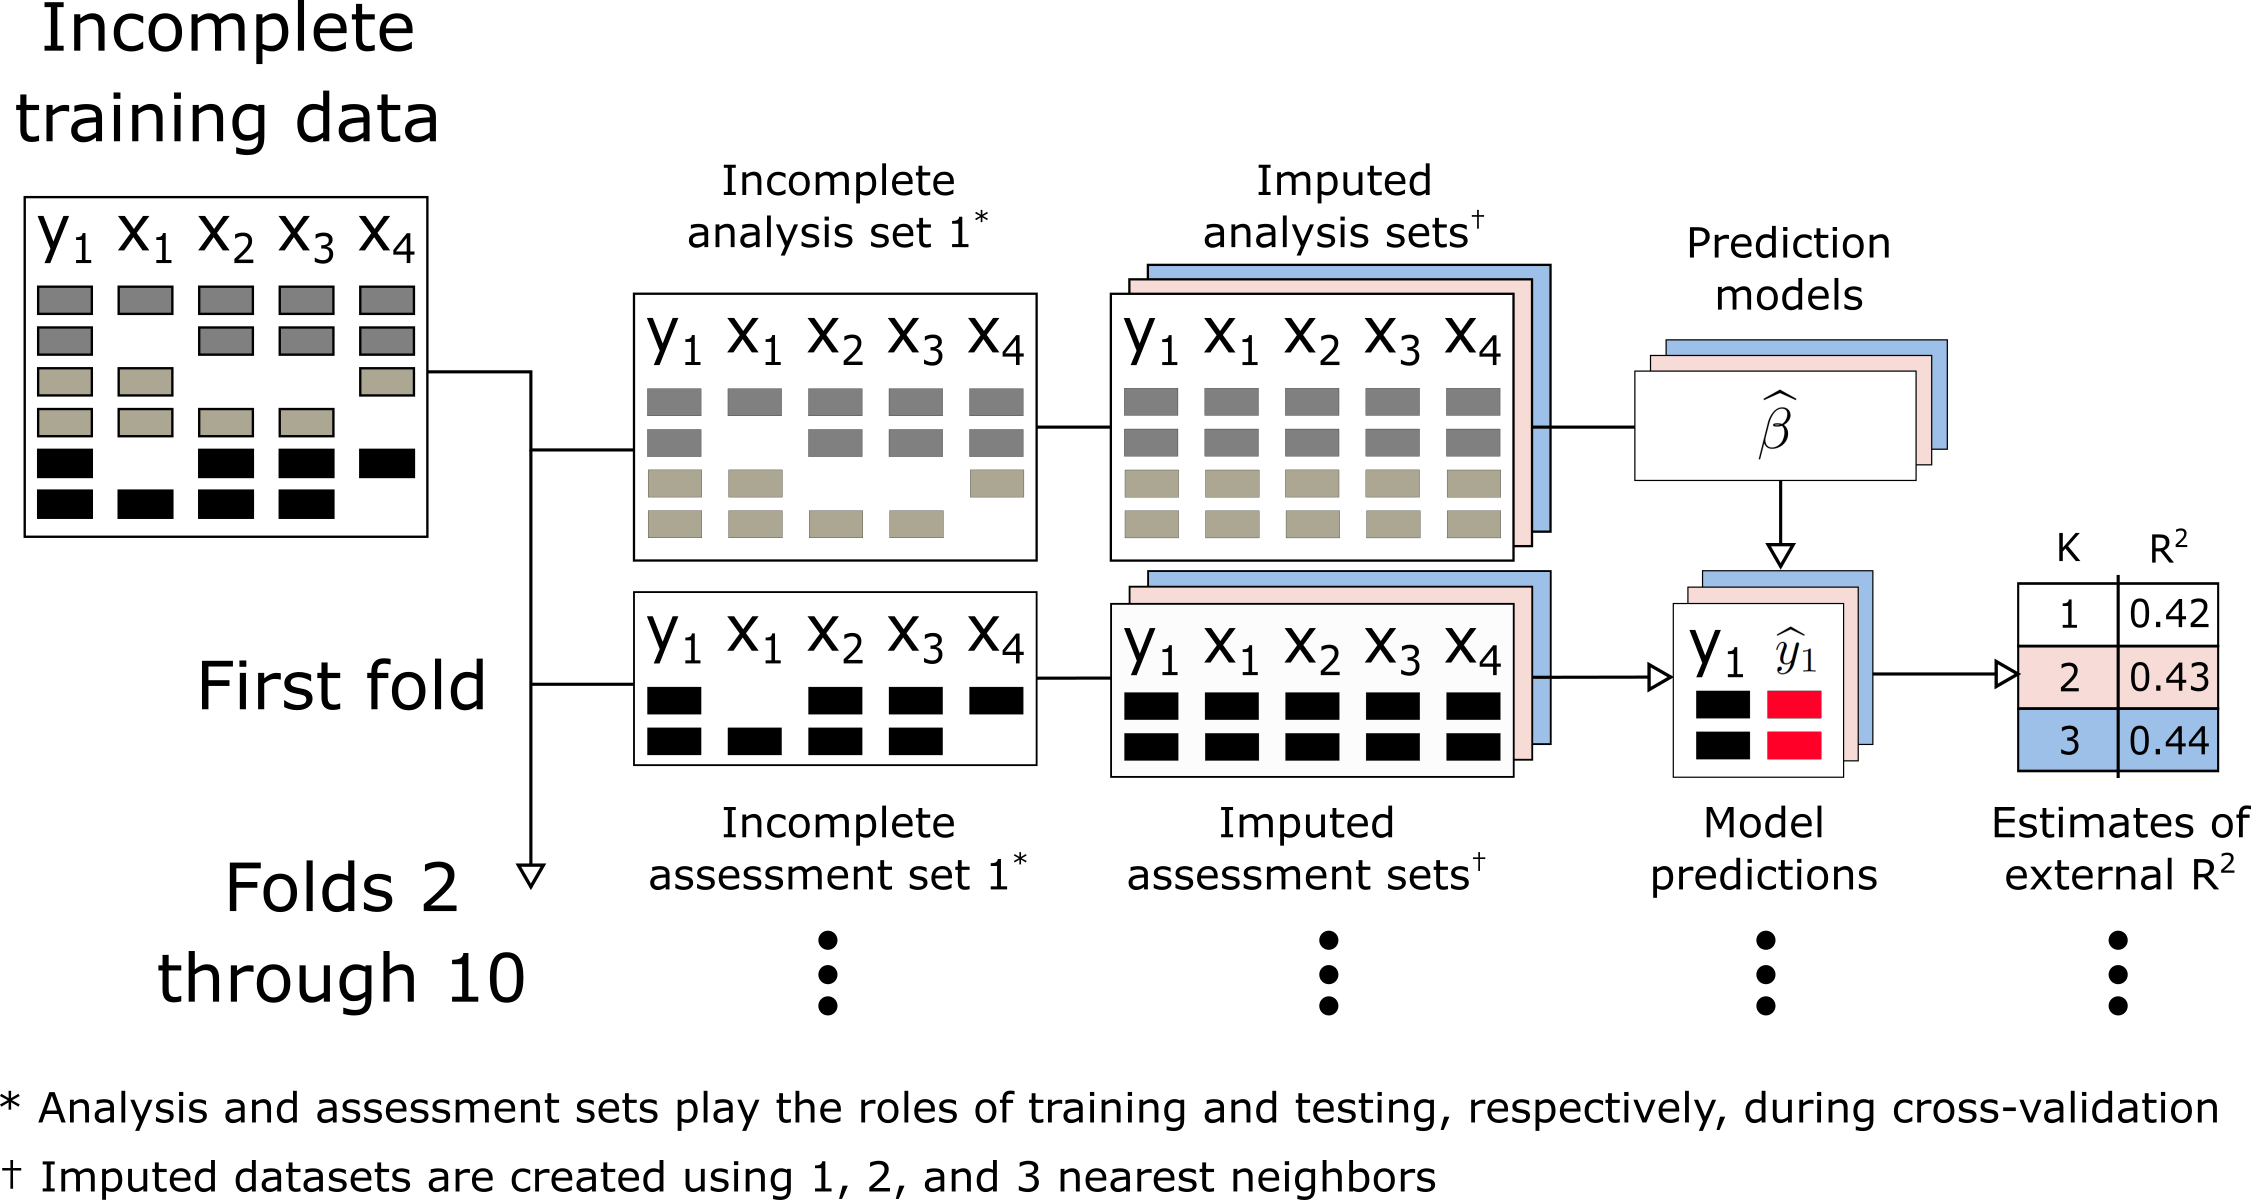
\includegraphics[width=1\linewidth]{figs/workflow_CVI} 
\caption{A traditional workflow for cross-validation that applies k-nearest neighbor unsupervised imputation within each replicate (\textit{i.e., }$\texttt{CV}\!\circlearrowright\!\texttt{I}$).}
\label{fig:workflow_cvi}
\end{figure}

\begin{figure}
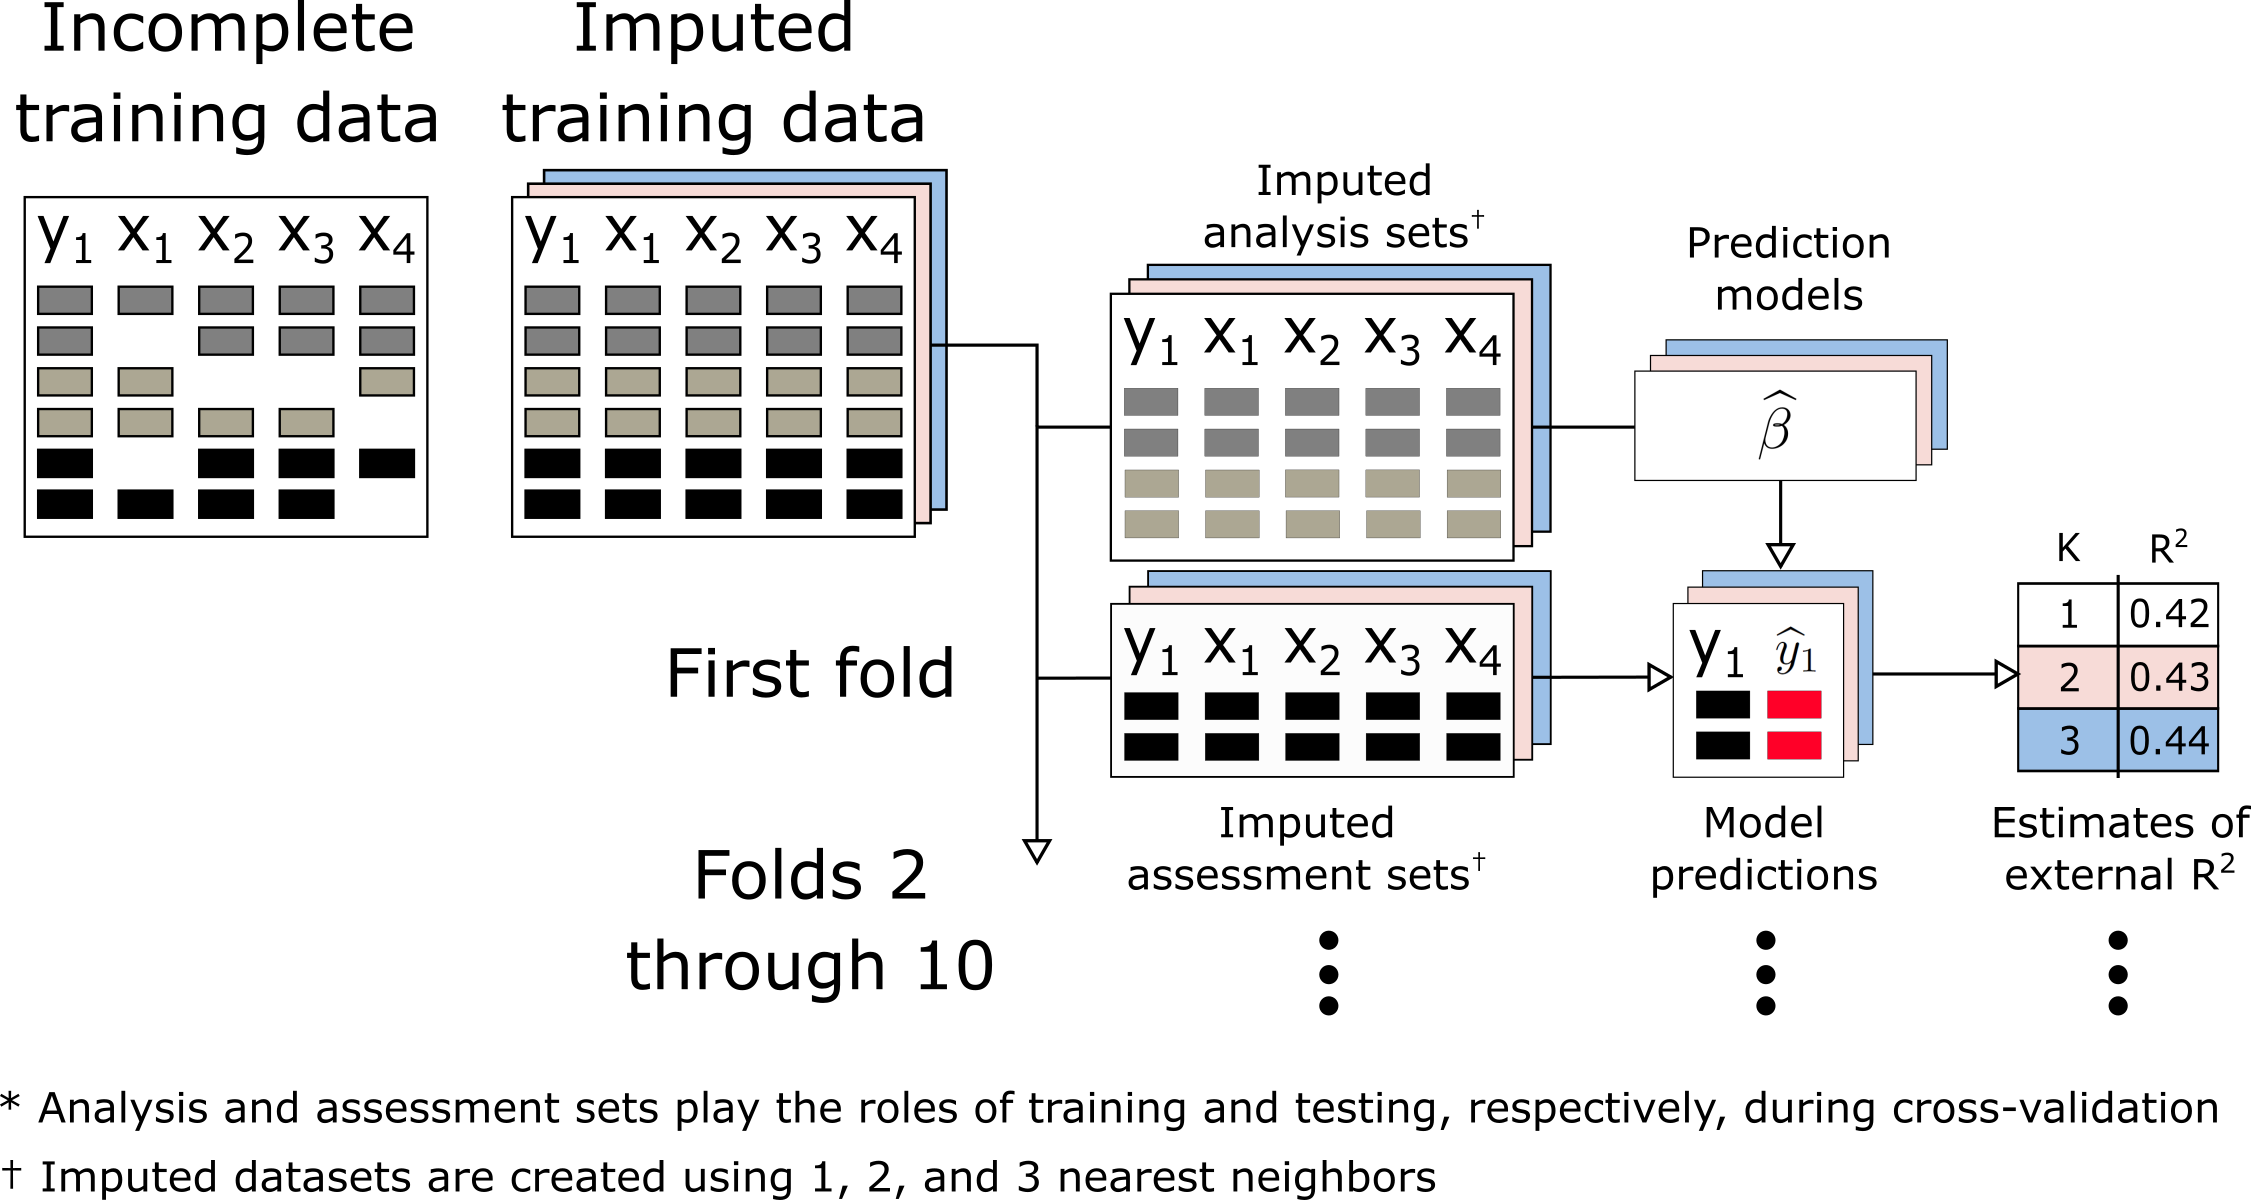
\includegraphics[width=1\linewidth]{figs/workflow_ICV} 
\caption{An experimental workflow for cross-validation that applies k-nearest neighbor unsupervised imputation prior to data splitting (\textit{i.e., }$\texttt{I}\!\!\rightarrow\!\texttt{CV}$)}
\label{fig:workflow_icv}
\end{figure}

\subsection{Testing data} \label{subsec:testing_data}

Ideally, external testing data will not contain MD, and imputation will
not be necessary. However, If MD are present in the external testing
data, additional steps may be taken to engage with them. One may impute
missing values in the testing data using (1) only the training data, (2)
only the testing data, or (3) using both training and testing data. It
is common to use only the training data to impute missing values in the
testing data. However, some imputation procedures can only impute values
in the data that were used to train the imputation procedure
(\textit{e.g., }matrix decomposition methods such as
\texttt{softImpute}).\citep{softImpute} To apply these types of
imputation procedures, approach (2) or (3) may be taken. In the current
analysis, $\texttt{CV}\!\circlearrowright\!\texttt{I}$\space uses only
the analysis data to impute missing values in the assessment data, and
$\texttt{I}\!\!\rightarrow\!\texttt{CV}$\space uses a stacked version of
the analysis and assessment data (\textit{i.e., }all of the training
data) to impute missing values. In the broader ML workflow (see Figure
\ref{fig:workflow_ml}), we employ approach (1), as is standard in
applied practice.

\section{Simulated experiments} \label{sec:sim}

The goal of the current simulation study was to assess empirical
differences between
$\texttt{CV}\!\circlearrowright\!\texttt{I}$\space and
$\texttt{I}\!\!\rightarrow\!\texttt{CV}$. Our primary objective was to
measure and compare how well each strategy (1) approximated a model's
generalization error and (2) selected parameters (both for imputation
and modeling) that would maximize downstream model accuracy. To complete
item (1), we assessed estimation of the oracle external \(R^2\). The
`oracle' performance is the performance of a model whose specification
coincides with the specification that generated the data the model is
fitted to. We used bias, variance, and root-mean-squared error (RMSE) to
quantify estimation accuracy. The RMSE provides an overall assessment of
estimation accuracy that depends on both bias and variance. To complete
item (2), we compared the performance (\textit{i.e., }the external
\(R^2\)) of downstream models whose tuning parameters were selected
using $\texttt{CV}\!\circlearrowright\!\texttt{I}$\space versus
$\texttt{I}\!\!\rightarrow\!\texttt{CV}$.

\subsection{Data-generating mechanisms} \label{subsec:data_gen}

Consider the linear regression model, where a continuous outcome vector
\(\textbf{y} = \lbrace y_1, y_2, \ldots, y_N\rbrace\) is generated by a
linear combination of predictor variables
\(\textbf{X} = \left[ \textbf{x}_1, \textbf{x}_2, \ldots \textbf{x}_p \right]\).
This functional relationship is often expressed as
\[\textbf{Y} = \textbf{X} \beta + \varepsilon,\] where \(\beta\) is a
\(p \times 1\) vector of regression coefficients and \(\varepsilon\) is
a normally distributed \(N \times 1\) zero-mean random error vector. In
practice, \(\textbf{X}\) often has some `junk' variables that are not
related to the outcome. We fixed the number of true predictor variables
at 10, the standard error of \(\varepsilon\) at 1, and set
\(\beta = [-1.00, -0.78, -0.56, -0.33, -0.11, 0.11, 0.33, 0.56, 0.78, 1.00]\)
throughout the simulation study. Columns of \(\textbf{X}\) were
generated from a multivariate normal distribution with a first order
autoregressive correlation structure. Specifically, the correlation
between columns \(\textbf{x}_i\) and \(\textbf{x}_j\) was
\(\rho^{\left| i-j \right|}\), where \(\rho\) was set to 3/4 throughout
the study. We applied this design to generate a training set of varying
size (100, 500, 1000, or 5000) along with an external validation set
comprising 10,000 observations in each simulated replicate.

We created three data-generation `scenarios'. In scenario 1, the
observed data are independent and identically distributed (iid). In
scenario 2, the data are iid conditional on an observed grouping
variable. A total of 11 groups are formed, one in the validation set and
the remaining 10 in the training set. Each group is characterized by a
randomly generated mean value for its predictor variables. During CV,
the observed groups are separated into ten folds to mimic the prediction
of outcomes in a population with different characteristics. Scenario 3
is identical to scenario 2 except that the grouping variable is latent.
Consequently, CV does not break the observed groups into separate folds
for scenario 3.

\paragraph{Amputing data}

We applied the \texttt{ampute} function from the \texttt{mice} R package
to generate missing values in simulated data. In each replicate, 90\% of
observations comprised at least one missing value. We designated up to
\(p\) MD patterns randomly in each simulation replicate, where \(p\) is
the number of non-outcome columns in the simulated data. A MD pattern
indicates which of the \(p\) predictor variables are set to missing. For
each MD pattern, the number of missing variables was randomly set to an
integer ranging from 1 to \(p/2\). This procedure usually induced
missing values in 30-50\% of the data. When data were MAR, we applied
the default method for the \texttt{ampute} function
(\texttt{ampute.default.weights}) to induce missingness based on the
observed variables. Throughout the experiment, we applied the same
missing patterns and MD mechanism in the training set and the external
validation set.

\paragraph{Modeling procedure}

We applied \(k\)-nearest-neighbor imputation to handle MD and least
absolute shrinkage and selection operator (LASSO) regression to develop
prediction functions throughout the simulated experiments. The LASSO
model is an `oracle' model for these simulations since all data were
generated with linear, independent effects. Nearest neighbor aggregation
was used to form imputed values in the training and testing set and also
in the analysis and assessment set for
$\texttt{CV}\!\circlearrowright\!\texttt{I}$. We created one imputed
dataset for each \(k \in \lbrace 1, 2, \ldots, 35\rbrace\). We selected
a value for the regularization parameter \(lambda\) in each imputed
dataset, separately, using 10-fold CV
(\textit{i.e., }\texttt{cv.glmnet}). The \(\lambda\) value selected was
the one that minimized the model's cross-validated RMSE. The value of
\(k\) that minimized cross-validated RMSE was used to impute the entire
training set prior to fitting a final \texttt{cv.glmnet} model.

\paragraph{Analysis plan}

We varied the scenario (1, 2, or 3; described in a preceding paragraph),
missing mechanism (MCAR or MAR), ratio of predictor variables to junk
variables (1:1, 1:4, and 1:49), and the number of training observations
(\(N\) = 100, 500, 1,000, 5,000). We present results for each of 72
settings determined by these parameters and also provide overall summary
statistics for scenarios 1, 2, and 3 when data are MCAR and MAR
(\textit{i.e., }aggregating over training sample size and predictor to
noise ratio). In each simulation replication, we computed the true
oracle external \(R^2\) in the validation set for each potential value
of nearest neighbors
(\textit{i.e., }\(k \in \lbrace 1, 2, \ldots, 35 \rbrace\)). {[}DEFINE
ORACLE{]} We also estimated external \(R^2\) for each value of \(k\)
using $\texttt{CV}\!\circlearrowright\!\texttt{I}$\space and
$\texttt{I}\!\!\rightarrow\!\texttt{CV}$, separately, to evaluate how
well these CV procedures estimated the true oracle external \(R^2\). We
assessed the difference between estimated external \(R^2\) according to
$\texttt{CV}\!\circlearrowright\!\texttt{I}$\space and
$\texttt{I}\!\!\rightarrow\!\texttt{CV}$\space as well as the bias,
variance, and root-mean-squared error (RMSE) of these estimates. Last,
we investigated the accuracy of downstream models when
$\texttt{CV}\!\circlearrowright\!\texttt{I}$\space and
$\texttt{I}\!\!\rightarrow\!\texttt{CV}$\space were applied to select
the number of neighbors to use for imputation and the regularization
parameter for a penalized regression model.

\subsection{Results} \label{subsec:sim_results}

Overall, a total of 143,253 out of 144,000 (99.5\%) simulation
replicates were completed over a span of 52,979 computing hours.
Incomplete replicates were not analyzed, as these were replicates where
at least one of the amputation, imputation, or prediction models did not
converge. Across all replicates, the mean number of minutes used to form
imputed data using
$\texttt{CV}\!\circlearrowright\!\texttt{I}$\space and
$\texttt{I}\!\!\rightarrow\!\texttt{CV}$\space were 7.42 and 0.80,
respectively, a ratio of 9.25. As a point of reference, using the full
training set, the mean number of minutes needed to tune and fit
\texttt{glmnet} models was 1.34.

Across all scenarios, the mean external \(R^2\) ranged from 0.233 to
0.443 (\textbf{Table} \ref{tab:ext_rsq}). External \(R^2\) values
increased with larger training set size and higher ratio of predictor
variables to junk variables. Notably, the mean external \(R^2\) values
in scenario 1 were uniformly greater than corresponding mean external
\(R^2\) values in scenarios 2 and 3, and the maximum difference between
mean external \(R^2\) values in scenario 2 versus scenario 3 was 0.0003.
The mean absolute difference between external \(R^2\) estimates using
$\texttt{CV}\!\circlearrowright\!\texttt{I}$\space and
$\texttt{I}\!\!\rightarrow\!\texttt{CV}$\space shrunk towards zero as
the size of the training set increased (\textbf{Table}
\ref{tab:cv_diffs}). The differences between
$\texttt{CV}\!\circlearrowright\!\texttt{I}$\space and
$\texttt{I}\!\!\rightarrow\!\texttt{CV}$\space were lowest in scenario 1
and greatest in scenario 2. These patterns were also present in visual
depictions of external \(R^2\) portrayed as a function of \(k\)
neighbors (\textbf{Figure} \ref{fig:sim_r2}).

\paragraph{Bias, variance, and RMSE}

For scenario 1, the overall bias of \(R^2\) estimates under MCAR using
$\texttt{CV}\!\circlearrowright\!\texttt{I}$\space was -0.00136 versus
0.00233 using
$\texttt{I}\!\!\rightarrow\!\texttt{CV}$\space (\textbf{Table}
\ref{tab:bias}). When the data were MAR, the overall biases were
-0.00080 for $\texttt{CV}\!\circlearrowright\!\texttt{I}$\space versus
0.00300 for $\texttt{I}\!\!\rightarrow\!\texttt{CV}$\space. In scenarios
2 and 3, the bias of
$\texttt{CV}\!\circlearrowright\!\texttt{I}$\space was lower than that
of $\texttt{I}\!\!\rightarrow\!\texttt{CV}$\space, and
$\texttt{I}\!\!\rightarrow\!\texttt{CV}$\space consistently provided
overly optimistic error estimates. The overall standard deviation of
\(R^2\) estimates was higher for
$\texttt{CV}\!\circlearrowright\!\texttt{I}$\space versus
$\texttt{I}\!\!\rightarrow\!\texttt{CV}$\space in all three scenarios
and both missing data mechanisms. The difference in standard deviation
was most pronounced in scenario 3 when data were MCAR (0.07314
{[}$\texttt{CV}\!\circlearrowright\!\texttt{I}${]} versus 0.06747
{[}$\texttt{I}\!\!\rightarrow\!\texttt{CV}${]}; \textbf{Table}
\ref{tab:variance}). Despite the optimistic bias of
$\texttt{I}\!\!\rightarrow\!\texttt{CV}$\space in scenario 2, the
reduced variance of this approach lead to a lower overall RMSE for
external \(R^2\) compared to
$\texttt{CV}\!\circlearrowright\!\texttt{I}$\space (\textbf{Table}
\ref{tab:rmse}). When the data were MCAR in scenario 2,
$\texttt{CV}\!\circlearrowright\!\texttt{I}$\space and
$\texttt{I}\!\!\rightarrow\!\texttt{CV}$\space obtained RMSEs of 0.05738
and 0.05593, respectively. Similarly, when the data were MAR in scenario
2, overall RMSE values were 0.05751 and 0.05572.

\paragraph{Downstream model performance}

When $\texttt{CV}\!\circlearrowright\!\texttt{I}$\space and
$\texttt{I}\!\!\rightarrow\!\texttt{CV}$\space were applied to select
tuning parameters, the overall mean external \(R^2\) was higher using
$\texttt{CV}\!\circlearrowright\!\texttt{I}$\space in 22 out of 78
comparisons (28\%; \textbf{Table} \ref{tab:tune}). The greatest overall
difference in mean \(R^2\) between downstream models occurred in
scenario 1 when the data were MAR (absolute difference in model \(R^2\):
0.00028; relative difference in model \(R^2\) : 0.07\%).

\section{Real data experiments} \label{sec:app}

The goal of the current resampling study was to repeat the comparisons
that were summarized in Section \ref{sec:sim} between
$\texttt{CV}\!\circlearrowright\!\texttt{I}$\space and
$\texttt{I}\!\!\rightarrow\!\texttt{CV}$\space using real, publicly
accessible data. A secondary objective was to assess how much results
would change if different modeling strategies were applied.

\paragraph{Ames, Iowa housing data}

The data we use in this resampling study describe the sale of individual
residential property in Ames, Iowa from 2006 to 2010. The entire set
contains 2930 observations and 80 variables (23 nominal, 23 ordinal, 14
discrete, and 20 continuous) that can be leveraged to predict the sale
price of homes.\cite{de2011ames} We used a cleaned version of the Ames
data for our own analyses by applying the \texttt{make\_ames()}
function, available in the \texttt{AmesHousing} R
package.\cite{AmesHousing} We also log-transformed the skewed sale price
outcome.

\paragraph{Analysis plan}

We conducted a resampling study where the Ames housing data was randomly
split into training (\(N = 2198\), 75\%) and testing (\(N = 732\), 25\%)
sets in each of 5,000 iterations. In each resampling replicate, we
implemented two separate modeling strategies to develop prediction
functions using the training set: (1) unpenalized linear regression and
(2) random forests. We also implemented two imputation strategies: (1)
nearest neighbor imputation using 1, 2, \ldots, 35 neighbors and (2)
mean and mode imputation for numeric and nominal variables,
respectively. In addition to imputation, data were pre-processed by
lumping values in discrete variables into an `other' category if the
value accounted for less than 10\% of the observed values. Both CV
techniques
(\textit{i.e., }$\texttt{CV}\!\circlearrowright\!\texttt{I}$\space and
$\texttt{I}\!\!\rightarrow\!\texttt{CV}$) were implemented to estimate
the external generalization error of the linear regression and random
forest models when nearest neighbor imputation was applied.

\paragraph{Amputing data}

The training and testing data were amputed in the same manner using four
prototypes of missingness. The prototypes were characterized by having
missing values for all variables describing the house (1) lot and
garage, (2) longitude and latitude, (3) basement and year built, and (4)
overall quality and general above ground square footage. We restricted
our prediction models to consider only the 30 predictor variables
belonging to at least one of these missing prototypes.

\subsection{Results}

A total of 5000 out of 5000 (100\%) resampling replicates were completed
over a span of 927 computing hours. Across all replicates, the mean
number of minutes used to form imputed data using
$\texttt{CV}\!\circlearrowright\!\texttt{I}$\space and
$\texttt{I}\!\!\rightarrow\!\texttt{CV}$\space were 10 and 1.0,
respectively. The mean (standard deviation) external \(R^2\) for the
linear regression and random forest models were 0.7641 (0.0265) and
0.8088 (0.0205), respectively. Overall, both CV techniques slightly over
and under estimated the external \(R^2\) value when linear regression
and random forests were applied, respectively. For linear regression,
the mean (standard deviation) bias was -0.0015 (0.0343) and -0.0021
(0.0343) for $\texttt{CV}\!\circlearrowright\!\texttt{I}$\space and
$\texttt{I}\!\!\rightarrow\!\texttt{CV}$, respectively. The standard
deviations of error estimates were 0.0115 and 0.0115, respectively. For
random forests, the mean (standard deviation) bias was 0.0009 (0.0255)
and 0.0005 (0.0255) for
$\texttt{CV}\!\circlearrowright\!\texttt{I}$\space and
$\texttt{I}\!\!\rightarrow\!\texttt{CV}$, respectively. The standard
deviation of error estimates were 0.0084 and 0.0086, respectively.

When $\texttt{CV}\!\circlearrowright\!\texttt{I}$\space and
$\texttt{I}\!\!\rightarrow\!\texttt{CV}$\space were applied to select
the number of neighbors used for imputation, downstream linear models
obtained an external \(R^2\) of 0.7657 (0.0260) and 0.7659 (0.0259),
respectively. Similarly, downstream random forests obtained an external
\(R^2\) of 0.8097 (0.0202) and 0.8096 (0.0201), respectively. As a
reference point, the mean (standard deviation) downstream external
\(R^2\) when imputation to the mean was applied was 0.7329 (0.0283) and
0.8127 (0.0199) using linear regression and random forests,
respectively.

\paragraph{Interpretation}

The use of $\texttt{CV}\!\circlearrowright\!\texttt{I}$\space versus
$\texttt{I}\!\!\rightarrow\!\texttt{CV}$\space resulted in a mean
relative change of 0.0262\% and -0.0220\% in downstream model
performance for linear models and random forests, respectively. These
shifts in model performance come at the cost of a \(v\)-fold increase in
the amount of computational resources allocated to handle MD. While
improvements on the order of hundredths of a percentage may be notable
for select analytic scenarios, these shifts in model performance may not
be relevant in the majority of supervised learning analyses. In the
latter case, it seems unsupervised imputation before CV can allow for
pragmatic handling of MD without sacrificing the integrity of CV.

\section{Discussion and recommendations} \label{sec:discuss}

We demonstrated empirical properties of
$\texttt{CV}\!\circlearrowright\!\texttt{I}$\space and
$\texttt{I}\!\!\rightarrow\!\texttt{CV}$\space using nearest-neighbor
imputation prior to applying regression and random forest models. We
selected these methods because they have been studied thoroughly and are
widely used in applied settings. In simulated experiments, we generated
outcomes using linear effects without interaction. We also studied three
broad scenarios that were relevant to CV: Scenario 1 was an ideal
setting where $\texttt{I}\!\!\rightarrow\!\texttt{CV}$\space and
$\texttt{CV}\!\circlearrowright\!\texttt{I}$\space should have provided
almost identical estimates of generalization error. Scenarios 2 and 3
were meant to test whether
$\texttt{I}\!\!\rightarrow\!\texttt{CV}$\space produced biased estimates
of generalization error because in settings where
$\texttt{I}\!\!\rightarrow\!\texttt{CV}$\space clearly did not mimic the
final application of a trained model to an external validation set.
Remarkably, despite its bias in scenario 2, the reduction in variance of
\(R^2\) estimates using
$\texttt{I}\!\!\rightarrow\!\texttt{CV}$\space lead to a lower overall
RMSE compared to $\texttt{CV}\!\circlearrowright\!\texttt{I}$.
Downstream model performance was consistently superior when
$\texttt{CV}\!\circlearrowright\!\texttt{I}$\space was used instead of
$\texttt{I}\!\!\rightarrow\!\texttt{CV}$. However, the increase in
performance was smaller than 1\% relative change (maximum overall
relative difference in external \(R^2\): 0.07\%). While this difference
is very small, it may be possible to find a different generative
scenario where the difference is larger.

Unsupervised imputation has two interesting characteristics relevant to
predictive modeling. First, it allows for imputation of testing data
whose outcome data are unobserved (not missing),
\textit{e.g., }predicting risk for incident cardiovascular disease among
adults with no history of cardiovascular disease. Second, as the current
analysis has shown, unsupervised imputation can be applied before CV in
select settings without inducing overly optimistic estimates of model
error. The benefits of this approach include (1) reduced computational
overhead, (2) reduced variance in model error estimates, and (3) little
difference in the performance of downstream models. If investigators are
confident that training and testing data are identically distributed or
are primarily concerned with selecting optimal tuning parameters,
$\texttt{I}\!\!\rightarrow\!\texttt{CV}$\space may be an extremely
convenient workflow to implement. However, the drawbacks of
$\texttt{I}\!\!\rightarrow\!\texttt{CV}$\space include increased bias
for model estimation, particularly in settings similar to scenario 2
(described in Section \ref{subsec:data_gen}). If investigators are
primarily interested in estimating model error without bias and cannot
rule out the possibility that testing data are drawn from a different
population or distribution than their training data, the current study
clearly suggests
$\texttt{CV}\!\circlearrowright\!\texttt{I}$\space should be applied
instead of $\texttt{I}\!\!\rightarrow\!\texttt{CV}$. However, it is
worth noting that almost all prediction modeling decisions require
balancing bias and variance to optimize precision. Our results do not
indicate any strong difference between
$\texttt{I}\!\!\rightarrow\!\texttt{CV}$\space and
$\texttt{CV}\!\circlearrowright\!\texttt{I}$with regard to precision
(\textit{i.e., }RMSE, see \textbf{Table} \ref{tab:rmse}). We suspect
that in most prediction modeling applications, precision rather than
bias is of primary interest.

The current study has several strengths. We implemented computational
experiments using real and simulated data. We included different
data-generation mechanisms, different modeling procedures, different MD
patterns, and different modeling strategies to ensure our results
generalized to several common analytical settings. We examined a wide
variety of metrics to assess the benefits and weaknesses of applying
$\texttt{I}\!\!\rightarrow\!\texttt{CV}$\space versus
$\texttt{CV}\!\circlearrowright\!\texttt{I}$. Last, we have provided (1)
an R package that conducts unsupervised imputation and (2) a github
repository disseminating all of the code necessary to reproduce our
results. Each of these supplemental components ensure that our work is
easily reproduced and disseminated. There are also some gaps in the
current study that can be filled by future work. We investigated
\(v\)-fold CV in the current analysis. Future research may assess
whether these results generalize to other forms of data-splitting such
as Monte-Carlo CV or bootstrap CV. Because MNAR data present challenges
that may not be overcome by imputation alone, we did not include
simulations for MNAR data. Whether the current study's findings
generalize to settings with MNAR data remains an interesting, unanswered
question. Last, the current study has applied k-nearest neighbor
imputation throughout. As many other types of imputation procedures have
been established, there are numerous extensions of the current analysis
that may explore whether our results hold when other imputation
approaches are implemented.

\FloatBarrier

\begin{table}

\caption{\label{tab:ext_rsq}True external $R^2$ values for the modeling technique that is internally assessed using $\texttt{CV}\!\circlearrowright\!\texttt{I}$\space and $\texttt{I}\!\!\rightarrow\!\texttt{CV}$.. All table values are scaled by 100 for convenience}
\centering
\begin{tabular}[t]{lcccccc}
\toprule
\multicolumn{1}{c}{ } & \multicolumn{2}{c}{Scenario 1} & \multicolumn{2}{c}{Scenario 2} & \multicolumn{2}{c}{Scenario 3} \\
\cmidrule(l{3pt}r{3pt}){2-3} \cmidrule(l{3pt}r{3pt}){4-5} \cmidrule(l{3pt}r{3pt}){6-7}
N & MAR & MCAR & MAR & MCAR & MAR & MCAR\\
\midrule
\addlinespace[0.75em]
\multicolumn{7}{l}{\textbf{10 predictors, 10 junk}}\\
\hline
\hspace{1em}100 & 37.8 (3.44) & 37.7 (3.43) & 33.5 (6.53) & 33.3 (6.69) & 33.5 (6.56) & 33.3 (6.69)\\
\hspace{1em}500 & 42.8 (2.91) & 42.7 (2.93) & 40.0 (4.97) & 39.8 (5.03) & 40.0 (4.98) & 39.8 (4.99)\\
\hspace{1em}1,000 & 43.5 (2.94) & 43.4 (2.95) & 40.9 (4.75) & 40.7 (4.80) & 40.9 (4.75) & 40.7 (4.79)\\
\hspace{1em}5,000 & 44.3 (3.01) & 44.2 (3.01) & 42.0 (4.46) & 41.8 (4.61) & 42.0 (4.46) & 41.8 (4.59)\\
\addlinespace[0.75em]
\multicolumn{7}{l}{\textbf{10 predictors, 40 junk}}\\
\hline
\hspace{1em}100 & 34.6 (3.83) & 34.5 (3.75) & 30.6 (6.39) & 30.6 (6.23) & 30.6 (6.44) & 30.5 (6.28)\\
\hspace{1em}500 & 40.6 (2.77) & 40.6 (2.77) & 38.2 (4.67) & 38.2 (4.73) & 38.2 (4.68) & 38.2 (4.61)\\
\hspace{1em}1,000 & 41.5 (2.73) & 41.5 (2.74) & 39.3 (4.68) & 39.2 (4.67) & 39.3 (4.67) & 39.2 (4.68)\\
\hspace{1em}5,000 & 42.6 (2.75) & 42.6 (2.75) & 40.6 (4.11) & 40.5 (4.17) & 40.6 (4.11) & 40.5 (4.20)\\
\addlinespace[0.75em]
\multicolumn{7}{l}{\textbf{10 predictors, 490 junk}}\\
\hline
\hspace{1em}100 & 27.5 (5.11) & 27.6 (5.03) & 23.3 (6.58) & 23.3 (6.47) & 23.3 (6.51) & 23.3 (6.47)\\
\hspace{1em}500 & 37.6 (2.93) & 37.6 (2.92) & 35.8 (4.09) & 35.9 (4.02) & 35.8 (4.09) & 35.9 (4.03)\\
\hspace{1em}1,000 & 38.8 (2.83) & 38.7 (2.83) & 37.2 (4.21) & 37.2 (4.22) & 37.2 (4.22) & 37.2 (4.23)\\
\hspace{1em}5,000 & 39.8 (2.78) & 39.8 (2.78) & 38.5 (4.06) & 38.5 (4.01) & 38.5 (4.05) & 38.5 (4.03)\\
\addlinespace[0.75em]
\multicolumn{7}{l}{\textbf{Overall}}\\
\hline
\hspace{1em}--- & 39.3 (5.51) & 39.2 (5.46) & 36.7 (7.18) & 36.6 (7.16) & 36.7 (7.17) & 36.6 (7.14)\\
\bottomrule
\end{tabular}
\end{table}

\begin{table}

\caption{\label{tab:cv_diffs}Mean absolute differences in estimates of external $R^2$ between $\texttt{CV}\!\circlearrowright\!\texttt{I}$\space and $\texttt{I}\!\!\rightarrow\!\texttt{CV}$.. All table values are scaled by 100 for convenience}
\centering
\begin{tabular}[t]{lcccccc}
\toprule
\multicolumn{1}{c}{ } & \multicolumn{2}{c}{Scenario 1} & \multicolumn{2}{c}{Scenario 2} & \multicolumn{2}{c}{Scenario 3} \\
\cmidrule(l{3pt}r{3pt}){2-3} \cmidrule(l{3pt}r{3pt}){4-5} \cmidrule(l{3pt}r{3pt}){6-7}
N & MAR & MCAR & MAR & MCAR & MAR & MCAR\\
\midrule
\addlinespace[0.75em]
\multicolumn{7}{l}{\textbf{10 predictors, 10 junk}}\\
\hline
\hspace{1em}100 & 1.21 (1.02) & 1.19 (0.99) & 2.43 (1.76) & 2.44 (1.79) & 2.05 (1.64) & 2.07 (1.67)\\
\hspace{1em}500 & 0.32 (0.29) & 0.33 (0.29) & 1.34 (1.13) & 1.39 (1.19) & 0.97 (1.05) & 1.00 (1.09)\\
\hspace{1em}1,000 & 0.21 (0.20) & 0.21 (0.20) & 1.22 (1.15) & 1.28 (1.21) & 0.87 (1.07) & 0.90 (1.12)\\
\hspace{1em}5,000 & 0.09 (0.08) & 0.09 (0.09) & 1.04 (0.92) & 1.09 (1.01) & 0.69 (0.89) & 0.71 (0.95)\\
\addlinespace[0.75em]
\multicolumn{7}{l}{\textbf{10 predictors, 40 junk}}\\
\hline
\hspace{1em}100 & 1.49 (1.27) & 1.47 (1.27) & 2.71 (1.97) & 2.67 (1.91) & 2.38 (1.89) & 2.35 (1.80)\\
\hspace{1em}500 & 0.33 (0.29) & 0.34 (0.29) & 1.40 (1.23) & 1.45 (1.29) & 1.01 (1.11) & 1.04 (1.17)\\
\hspace{1em}1,000 & 0.22 (0.20) & 0.22 (0.20) & 1.27 (1.16) & 1.33 (1.23) & 0.90 (1.09) & 0.93 (1.15)\\
\hspace{1em}5,000 & 0.09 (0.09) & 0.10 (0.09) & 1.15 (1.06) & 1.23 (1.16) & 0.77 (1.01) & 0.80 (1.08)\\
\addlinespace[0.75em]
\multicolumn{7}{l}{\textbf{10 predictors, 490 junk}}\\
\hline
\hspace{1em}100 & 2.09 (1.73) & 2.02 (1.67) & 3.01 (2.18) & 3.01 (2.14) & 2.75 (2.04) & 2.79 (2.05)\\
\hspace{1em}500 & 0.34 (0.29) & 0.34 (0.29) & 1.21 (1.15) & 1.21 (1.14) & 0.88 (1.05) & 0.89 (1.05)\\
\hspace{1em}1,000 & 0.21 (0.19) & 0.21 (0.19) & 1.16 (1.16) & 1.15 (1.15) & 0.81 (1.04) & 0.79 (1.02)\\
\hspace{1em}5,000 & 0.09 (0.08) & 0.09 (0.08) & 1.12 (1.11) & 1.18 (1.17) & 0.74 (1.03) & 0.77 (1.08)\\
\addlinespace[0.75em]
\multicolumn{7}{l}{\textbf{Overall}}\\
\hline
\hspace{1em}--- & 0.56 (0.95) & 0.55 (0.93) & 1.59 (1.54) & 1.62 (1.55) & 1.23 (1.47) & 1.25 (1.48)\\
\bottomrule
\end{tabular}
\end{table}

\begin{table}

\caption{\label{tab:bias}Bias of external $R^2$ estimates using $\texttt{CV}\!\circlearrowright\!\texttt{I}$\space and $\texttt{I}\!\!\rightarrow\!\texttt{CV}$.. All table values are scaled by 100 for convenience}
\centering
\begin{tabular}[t]{lcccccccccccc}
\toprule
\multicolumn{1}{c}{ } & \multicolumn{6}{c}{Missing completely at random} & \multicolumn{6}{c}{Missing at random} \\
\cmidrule(l{3pt}r{3pt}){2-7} \cmidrule(l{3pt}r{3pt}){8-13}
\multicolumn{1}{c}{ } & \multicolumn{2}{c}{Scenario 1} & \multicolumn{2}{c}{Scenario 2} & \multicolumn{2}{c}{Scenario 3} & \multicolumn{2}{c}{Scenario 1} & \multicolumn{2}{c}{Scenario 2} & \multicolumn{2}{c}{Scenario 3} \\
\cmidrule(l{3pt}r{3pt}){2-3} \cmidrule(l{3pt}r{3pt}){4-5} \cmidrule(l{3pt}r{3pt}){6-7} \cmidrule(l{3pt}r{3pt}){8-9} \cmidrule(l{3pt}r{3pt}){10-11} \cmidrule(l{3pt}r{3pt}){12-13}
N & $\texttt{CV}\!\circlearrowright\!\texttt{I}$& $\texttt{I}\!\!\rightarrow\!\texttt{CV}$& $\texttt{CV}\!\circlearrowright\!\texttt{I}$& $\texttt{I}\!\!\rightarrow\!\texttt{CV}$& $\texttt{CV}\!\circlearrowright\!\texttt{I}$& $\texttt{I}\!\!\rightarrow\!\texttt{CV}$& $\texttt{CV}\!\circlearrowright\!\texttt{I}$& $\texttt{I}\!\!\rightarrow\!\texttt{CV}$& $\texttt{CV}\!\circlearrowright\!\texttt{I}$& $\texttt{I}\!\!\rightarrow\!\texttt{CV}$& $\texttt{CV}\!\circlearrowright\!\texttt{I}$& $\texttt{I}\!\!\rightarrow\!\texttt{CV}$\\
\midrule
\addlinespace[0.75em]
\multicolumn{13}{l}{\textbf{10 predictors, 10 junk}}\\
\hline
\hspace{1em}100 & 0.31 & -0.48 & 1.06 & -1.14 & 0.57 & -1.21 & 0.51 & -0.31 & 1.32 & -0.85 & 0.76 & -0.99\\
\hspace{1em}500 & 0.10 & -0.02 & 0.26 & -1.06 & -0.20 & -1.07 & 0.11 & 0.01 & 0.41 & -0.86 & -0.05 & -0.90\\
\hspace{1em}1,000 & 0.09 & 0.04 & 0.20 & -1.04 & -0.26 & -1.08 & 0.10 & 0.04 & 0.36 & -0.83 & -0.08 & -0.87\\
\hspace{1em}5,000 & 0.00 & 0.00 & 0.11 & -0.97 & -0.32 & -0.99 & 0.01 & 0.00 & 0.28 & -0.75 & -0.11 & -0.77\\
\addlinespace[0.75em]
\multicolumn{13}{l}{\textbf{10 predictors, 40 junk}}\\
\hline
\hspace{1em}100 & 0.62 & -0.52 & 1.02 & -1.44 & 0.56 & -1.56 & 0.80 & -0.39 & 1.33 & -1.17 & 0.82 & -1.31\\
\hspace{1em}500 & 0.14 & -0.01 & 0.36 & -1.01 & -0.09 & -1.02 & 0.20 & 0.07 & 0.45 & -0.88 & -0.02 & -0.91\\
\hspace{1em}1,000 & 0.04 & -0.04 & 0.19 & -1.11 & -0.29 & -1.15 & 0.06 & -0.02 & 0.22 & -1.02 & -0.22 & -1.04\\
\hspace{1em}5,000 & 0.06 & 0.03 & 0.16 & -1.06 & -0.31 & -1.09 & 0.05 & 0.03 & 0.22 & -0.92 & -0.20 & -0.94\\
\addlinespace[0.75em]
\multicolumn{13}{l}{\textbf{10 predictors, 490 junk}}\\
\hline
\hspace{1em}100 & 1.08 & -0.74 & 1.44 & -1.43 & 1.26 & -1.39 & 1.02 & -0.88 & 1.42 & -1.46 & 1.15 & -1.46\\
\hspace{1em}500 & 0.23 & 0.08 & 0.38 & -0.68 & 0.02 & -0.70 & 0.37 & 0.21 & 0.48 & -0.58 & 0.11 & -0.61\\
\hspace{1em}1,000 & 0.12 & 0.06 & 0.20 & -0.87 & -0.20 & -0.88 & 0.31 & 0.24 & 0.38 & -0.68 & -0.01 & -0.71\\
\hspace{1em}5,000 & 0.00 & -0.02 & 0.26 & -0.90 & -0.20 & -0.93 & 0.05 & 0.03 & 0.26 & -0.85 & -0.16 & -0.86\\
\addlinespace[0.75em]
\multicolumn{13}{l}{\textbf{Overall}}\\
\hline
\hspace{1em}--- & 0.23 & -0.14 & 0.47 & -1.06 & 0.04 & -1.09 & 0.30 & -0.08 & 0.59 & -0.90 & 0.16 & -0.95\\
\bottomrule
\end{tabular}
\end{table}

\begin{table}

\caption{\label{tab:variance}Standard deviation of external $R^2$ estimates using $\texttt{CV}\!\circlearrowright\!\texttt{I}$\space and $\texttt{I}\!\!\rightarrow\!\texttt{CV}$.. All table values are scaled by 100 for convenience}
\centering
\begin{tabular}[t]{lcccccccccccc}
\toprule
\multicolumn{1}{c}{ } & \multicolumn{6}{c}{Missing completely at random} & \multicolumn{6}{c}{Missing at random} \\
\cmidrule(l{3pt}r{3pt}){2-7} \cmidrule(l{3pt}r{3pt}){8-13}
\multicolumn{1}{c}{ } & \multicolumn{2}{c}{Scenario 1} & \multicolumn{2}{c}{Scenario 2} & \multicolumn{2}{c}{Scenario 3} & \multicolumn{2}{c}{Scenario 1} & \multicolumn{2}{c}{Scenario 2} & \multicolumn{2}{c}{Scenario 3} \\
\cmidrule(l{3pt}r{3pt}){2-3} \cmidrule(l{3pt}r{3pt}){4-5} \cmidrule(l{3pt}r{3pt}){6-7} \cmidrule(l{3pt}r{3pt}){8-9} \cmidrule(l{3pt}r{3pt}){10-11} \cmidrule(l{3pt}r{3pt}){12-13}
N & $\texttt{CV}\!\circlearrowright\!\texttt{I}$& $\texttt{I}\!\!\rightarrow\!\texttt{CV}$& $\texttt{CV}\!\circlearrowright\!\texttt{I}$& $\texttt{I}\!\!\rightarrow\!\texttt{CV}$& $\texttt{CV}\!\circlearrowright\!\texttt{I}$& $\texttt{I}\!\!\rightarrow\!\texttt{CV}$& $\texttt{CV}\!\circlearrowright\!\texttt{I}$& $\texttt{I}\!\!\rightarrow\!\texttt{CV}$& $\texttt{CV}\!\circlearrowright\!\texttt{I}$& $\texttt{I}\!\!\rightarrow\!\texttt{CV}$& $\texttt{CV}\!\circlearrowright\!\texttt{I}$& $\texttt{I}\!\!\rightarrow\!\texttt{CV}$\\
\midrule
\addlinespace[0.75em]
\multicolumn{13}{l}{\textbf{10 predictors, 10 junk}}\\
\hline
\hspace{1em}100 & 6.41 & 6.38 & 7.56 & 7.09 & 7.46 & 7.04 & 6.37 & 6.33 & 7.52 & 7.13 & 7.44 & 7.06\\
\hspace{1em}500 & 3.59 & 3.64 & 3.92 & 3.82 & 3.92 & 3.81 & 3.60 & 3.65 & 3.92 & 3.82 & 3.91 & 3.81\\
\hspace{1em}1,000 & 3.32 & 3.36 & 3.67 & 3.55 & 3.65 & 3.54 & 3.31 & 3.35 & 3.67 & 3.55 & 3.65 & 3.54\\
\hspace{1em}5,000 & 3.08 & 3.10 & 3.39 & 3.29 & 3.40 & 3.28 & 3.07 & 3.09 & 3.37 & 3.28 & 3.38 & 3.27\\
\addlinespace[0.75em]
\multicolumn{13}{l}{\textbf{10 predictors, 40 junk}}\\
\hline
\hspace{1em}100 & 6.73 & 6.62 & 7.28 & 6.91 & 7.19 & 6.88 & 6.62 & 6.51 & 7.30 & 6.89 & 7.23 & 6.85\\
\hspace{1em}500 & 3.55 & 3.60 & 3.75 & 3.65 & 3.70 & 3.65 & 3.57 & 3.61 & 3.73 & 3.64 & 3.71 & 3.65\\
\hspace{1em}1,000 & 3.14 & 3.17 & 3.31 & 3.22 & 3.32 & 3.21 & 3.16 & 3.19 & 3.28 & 3.21 & 3.31 & 3.21\\
\hspace{1em}5,000 & 2.82 & 2.84 & 3.02 & 2.89 & 3.02 & 2.89 & 2.82 & 2.84 & 2.99 & 2.88 & 3.00 & 2.88\\
\addlinespace[0.75em]
\multicolumn{13}{l}{\textbf{10 predictors, 490 junk}}\\
\hline
\hspace{1em}100 & 7.66 & 7.43 & 7.89 & 7.51 & 7.84 & 7.50 & 7.52 & 7.31 & 8.00 & 7.61 & 7.96 & 7.56\\
\hspace{1em}500 & 3.69 & 3.73 & 3.85 & 3.78 & 3.86 & 3.78 & 3.72 & 3.75 & 3.85 & 3.77 & 3.87 & 3.78\\
\hspace{1em}1,000 & 3.26 & 3.29 & 3.30 & 3.21 & 3.30 & 3.21 & 3.27 & 3.29 & 3.33 & 3.24 & 3.34 & 3.25\\
\hspace{1em}5,000 & 2.86 & 2.87 & 2.95 & 2.87 & 2.98 & 2.87 & 2.87 & 2.88 & 2.94 & 2.87 & 2.97 & 2.88\\
\addlinespace[0.75em]
\multicolumn{13}{l}{\textbf{Overall}}\\
\hline
\hspace{1em}--- & 6.50 & 6.12 & 7.31 & 6.77 & 7.31 & 6.75 & 6.52 & 6.12 & 7.34 & 6.79 & 7.33 & 6.76\\
\bottomrule
\end{tabular}
\end{table}

\begin{table}

\caption{\label{tab:rmse}Root-mean-squared error of external $R^2$ estimates using $\texttt{CV}\!\circlearrowright\!\texttt{I}$\space and $\texttt{I}\!\!\rightarrow\!\texttt{CV}$.. All table values are scaled by 100 for convenience}
\centering
\begin{tabular}[t]{lcccccccccccc}
\toprule
\multicolumn{1}{c}{ } & \multicolumn{6}{c}{Missing completely at random} & \multicolumn{6}{c}{Missing at random} \\
\cmidrule(l{3pt}r{3pt}){2-7} \cmidrule(l{3pt}r{3pt}){8-13}
\multicolumn{1}{c}{ } & \multicolumn{2}{c}{Scenario 1} & \multicolumn{2}{c}{Scenario 2} & \multicolumn{2}{c}{Scenario 3} & \multicolumn{2}{c}{Scenario 1} & \multicolumn{2}{c}{Scenario 2} & \multicolumn{2}{c}{Scenario 3} \\
\cmidrule(l{3pt}r{3pt}){2-3} \cmidrule(l{3pt}r{3pt}){4-5} \cmidrule(l{3pt}r{3pt}){6-7} \cmidrule(l{3pt}r{3pt}){8-9} \cmidrule(l{3pt}r{3pt}){10-11} \cmidrule(l{3pt}r{3pt}){12-13}
N & $\texttt{CV}\!\circlearrowright\!\texttt{I}$& $\texttt{I}\!\!\rightarrow\!\texttt{CV}$& $\texttt{CV}\!\circlearrowright\!\texttt{I}$& $\texttt{I}\!\!\rightarrow\!\texttt{CV}$& $\texttt{CV}\!\circlearrowright\!\texttt{I}$& $\texttt{I}\!\!\rightarrow\!\texttt{CV}$& $\texttt{CV}\!\circlearrowright\!\texttt{I}$& $\texttt{I}\!\!\rightarrow\!\texttt{CV}$& $\texttt{CV}\!\circlearrowright\!\texttt{I}$& $\texttt{I}\!\!\rightarrow\!\texttt{CV}$& $\texttt{CV}\!\circlearrowright\!\texttt{I}$& $\texttt{I}\!\!\rightarrow\!\texttt{CV}$\\
\midrule
\addlinespace[0.75em]
\multicolumn{13}{l}{\textbf{10 predictors, 10 junk}}\\
\hline
\hspace{1em}100 & 5.93 & 5.86 & 9.08 & 8.74 & 8.94 & 8.69 & 5.87 & 5.77 & 8.98 & 8.62 & 8.84 & 8.59\\
\hspace{1em}500 & 2.22 & 2.22 & 4.98 & 4.91 & 4.91 & 4.86 & 2.22 & 2.22 & 4.94 & 4.84 & 4.92 & 4.85\\
\hspace{1em}1,000 & 1.64 & 1.64 & 4.31 & 4.20 & 4.25 & 4.22 & 1.64 & 1.64 & 4.25 & 4.11 & 4.19 & 4.12\\
\hspace{1em}5,000 & 0.82 & 0.82 & 3.67 & 3.63 & 3.64 & 3.61 & 0.82 & 0.82 & 3.48 & 3.40 & 3.46 & 3.40\\
\addlinespace[0.75em]
\multicolumn{13}{l}{\textbf{10 predictors, 40 junk}}\\
\hline
\hspace{1em}100 & 6.36 & 6.26 & 8.77 & 8.53 & 8.72 & 8.59 & 6.36 & 6.23 & 8.97 & 8.64 & 8.92 & 8.68\\
\hspace{1em}500 & 2.36 & 2.36 & 4.79 & 4.69 & 4.61 & 4.59 & 2.34 & 2.33 & 4.74 & 4.61 & 4.66 & 4.62\\
\hspace{1em}1,000 & 1.66 & 1.66 & 4.39 & 4.37 & 4.39 & 4.39 & 1.69 & 1.69 & 4.42 & 4.37 & 4.39 & 4.37\\
\hspace{1em}5,000 & 0.82 & 0.82 & 3.58 & 3.48 & 3.59 & 3.52 & 0.81 & 0.81 & 3.45 & 3.35 & 3.44 & 3.36\\
\addlinespace[0.75em]
\multicolumn{13}{l}{\textbf{10 predictors, 490 junk}}\\
\hline
\hspace{1em}100 & 7.38 & 7.31 & 8.93 & 8.79 & 8.90 & 8.80 & 7.35 & 7.35 & 9.06 & 8.89 & 8.91 & 8.80\\
\hspace{1em}500 & 2.43 & 2.42 & 4.17 & 4.01 & 4.14 & 4.02 & 2.45 & 2.43 & 4.24 & 4.05 & 4.21 & 4.07\\
\hspace{1em}1,000 & 1.76 & 1.75 & 3.91 & 3.78 & 3.89 & 3.80 & 1.76 & 1.75 & 3.92 & 3.72 & 3.87 & 3.75\\
\hspace{1em}5,000 & 0.85 & 0.85 & 3.38 & 3.24 & 3.37 & 3.27 & 0.86 & 0.86 & 3.42 & 3.28 & 3.38 & 3.28\\
\addlinespace[0.75em]
\multicolumn{13}{l}{\textbf{Overall}}\\
\hline
\hspace{1em}--- & 3.62 & 3.58 & 5.74 & 5.59 & 5.68 & 5.59 & 3.61 & 3.57 & 5.75 & 5.57 & 5.68 & 5.56\\
\bottomrule
\end{tabular}
\end{table}

\begin{table}

\caption{\label{tab:tune}Mean external $R^2$ when $\texttt{CV}\!\circlearrowright\!\texttt{I}$\space and $\texttt{I}\!\!\rightarrow\!\texttt{CV}$\space were applied to tune the number of neighbors used for imputation.. All table values are scaled by 100 for convenience}
\centering
\begin{tabular}[t]{lcccccccccccc}
\toprule
\multicolumn{1}{c}{ } & \multicolumn{6}{c}{Missing completely at random} & \multicolumn{6}{c}{Missing at random} \\
\cmidrule(l{3pt}r{3pt}){2-7} \cmidrule(l{3pt}r{3pt}){8-13}
\multicolumn{1}{c}{ } & \multicolumn{2}{c}{Scenario 1} & \multicolumn{2}{c}{Scenario 2} & \multicolumn{2}{c}{Scenario 3} & \multicolumn{2}{c}{Scenario 1} & \multicolumn{2}{c}{Scenario 2} & \multicolumn{2}{c}{Scenario 3} \\
\cmidrule(l{3pt}r{3pt}){2-3} \cmidrule(l{3pt}r{3pt}){4-5} \cmidrule(l{3pt}r{3pt}){6-7} \cmidrule(l{3pt}r{3pt}){8-9} \cmidrule(l{3pt}r{3pt}){10-11} \cmidrule(l{3pt}r{3pt}){12-13}
N & $\texttt{CV}\!\circlearrowright\!\texttt{I}$& $\texttt{I}\!\!\rightarrow\!\texttt{CV}$& $\texttt{CV}\!\circlearrowright\!\texttt{I}$& $\texttt{I}\!\!\rightarrow\!\texttt{CV}$& $\texttt{CV}\!\circlearrowright\!\texttt{I}$& $\texttt{I}\!\!\rightarrow\!\texttt{CV}$& $\texttt{CV}\!\circlearrowright\!\texttt{I}$& $\texttt{I}\!\!\rightarrow\!\texttt{CV}$& $\texttt{CV}\!\circlearrowright\!\texttt{I}$& $\texttt{I}\!\!\rightarrow\!\texttt{CV}$& $\texttt{CV}\!\circlearrowright\!\texttt{I}$& $\texttt{I}\!\!\rightarrow\!\texttt{CV}$\\
\midrule
\addlinespace[0.75em]
\multicolumn{13}{l}{\textbf{10 predictors, 10 junk}}\\
\hline
\hspace{1em}100 & 38.1 & 38.1 & 33.9 & 34.0 & 34.0 & 34.0 & 38.3 & 38.3 & 34.2 & 34.2 & 34.1 & 34.1\\
\hspace{1em}500 & 43.8 & 43.8 & 40.7 & 40.8 & 40.8 & 40.8 & 43.9 & 43.9 & 41.0 & 41.0 & 41.0 & 41.0\\
\hspace{1em}1,000 & 44.7 & 44.8 & 41.9 & 41.9 & 41.9 & 41.9 & 44.8 & 44.8 & 42.1 & 42.1 & 42.1 & 42.1\\
\hspace{1em}5,000 & 45.7 & 45.7 & 43.3 & 43.3 & 43.3 & 43.3 & 45.8 & 45.8 & 43.5 & 43.5 & 43.5 & 43.5\\
\addlinespace[0.75em]
\multicolumn{13}{l}{\textbf{10 predictors, 40 junk}}\\
\hline
\hspace{1em}100 & 35.1 & 35.0 & 31.1 & 31.2 & 31.1 & 31.1 & 35.2 & 35.0 & 31.1 & 31.0 & 31.1 & 31.1\\
\hspace{1em}500 & 41.8 & 41.8 & 39.1 & 39.2 & 39.2 & 39.2 & 41.8 & 41.8 & 39.2 & 39.2 & 39.2 & 39.2\\
\hspace{1em}1,000 & 42.8 & 42.8 & 40.3 & 40.3 & 40.3 & 40.3 & 42.8 & 42.8 & 40.4 & 40.4 & 40.4 & 40.4\\
\hspace{1em}5,000 & 44.0 & 44.0 & 41.9 & 41.9 & 41.9 & 41.9 & 44.0 & 44.0 & 42.0 & 42.0 & 42.0 & 42.0\\
\addlinespace[0.75em]
\multicolumn{13}{l}{\textbf{10 predictors, 490 junk}}\\
\hline
\hspace{1em}100 & 28.8 & 28.5 & 24.0 & 23.7 & 24.0 & 23.7 & 28.6 & 28.4 & 24.1 & 23.8 & 24.2 & 23.9\\
\hspace{1em}500 & 39.1 & 39.1 & 37.2 & 37.3 & 37.2 & 37.3 & 39.1 & 39.1 & 37.2 & 37.3 & 37.2 & 37.2\\
\hspace{1em}1,000 & 40.4 & 40.4 & 38.7 & 38.7 & 38.7 & 38.7 & 40.4 & 40.4 & 38.7 & 38.7 & 38.7 & 38.7\\
\hspace{1em}5,000 & 41.5 & 41.5 & 40.1 & 40.1 & 40.1 & 40.1 & 41.5 & 41.5 & 40.1 & 40.1 & 40.1 & 40.1\\
\addlinespace[0.75em]
\multicolumn{13}{l}{\textbf{Overall}}\\
\hline
\hspace{1em}--- & 40.5 & 40.5 & 37.7 & 37.7 & 37.7 & 37.7 & 40.5 & 40.5 & 37.8 & 37.8 & 37.8 & 37.8\\
\bottomrule
\end{tabular}
\end{table}

\begin{figure}
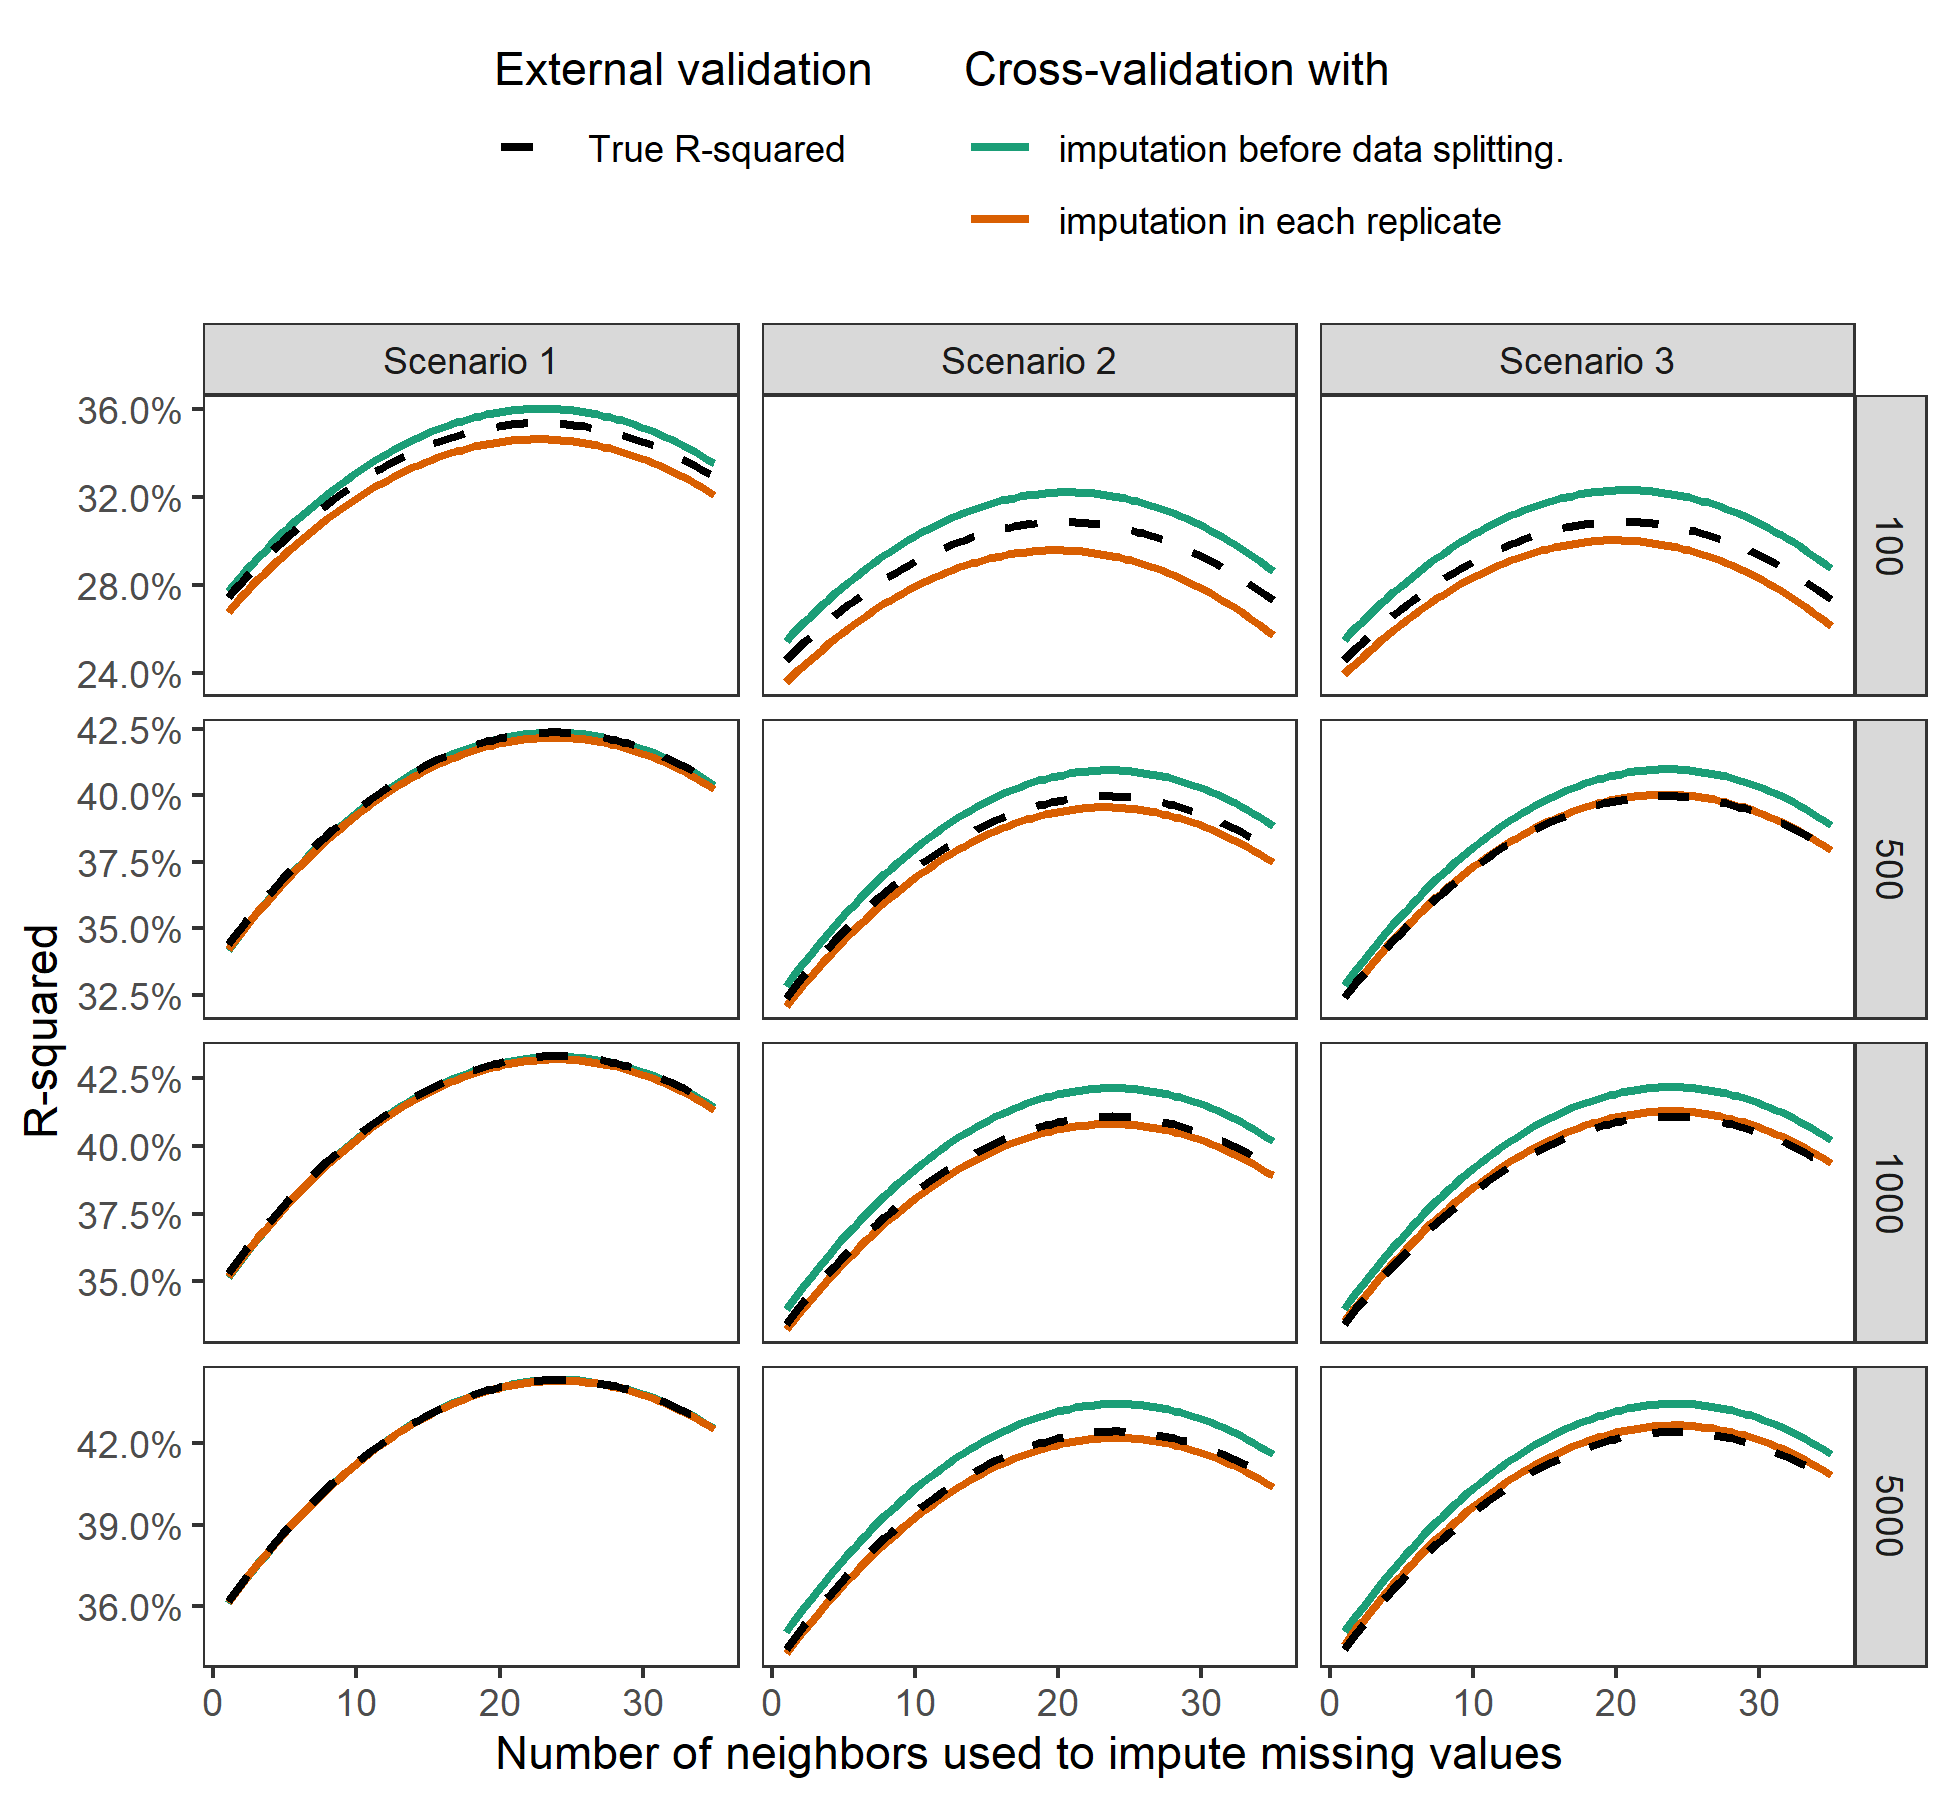
\includegraphics[width=1\linewidth]{figs/fig_trends_by_nbrs} 
\caption{External generalization error and internal estimates of generalization error using $\texttt{I}\!\!\rightarrow\!\texttt{CV}$\space and $\texttt{CV}\!\circlearrowright\!\texttt{I}$.}
\label{fig:sim_r2}
\end{figure}

\FloatBarrier

\bibliography{bibfile.bib}


\end{document}
